  \section{Hardware}
  Hardware implementering af \textit{The Cell Collector} består af enhedstest af hver komponent, med følgende dokumentation. Enhedstestende er lavet i den skrevne rækkefølge og integreret i samme. I dette afsnit vil der være kredsløbsdiagrammer, teori, formler og beskrivelser. Hvilket er udarbejdet sideløbende med udviklingen af produktet. 
 
 \subsection{Vægtcelle}
 For at kunne udnytte funktionen af en vægtcelle, skal opbygningen af denne forstås. En vægtcelle måler hvor meget vægt den udsættes for, vægcellen som den type der er brugt i dette projekt består af strain gages koblet i en wheatstone bro. En strain gages bruges til at måle fysisk stræk eller kompression. Den er simpel i sin opbygning ved at består af en meget tynd elektrisk ledende tråd, som er ført frem og tilbage på et elastisk folie, hvilket er illustreret på \ref{fig:Strain gages}\footnote{billedet er hentet med tilladelse fra  \url{https://en.wikipedia.org/wiki/Strain_gauge}}. 
 \begin{figure}[H]
	\centering
	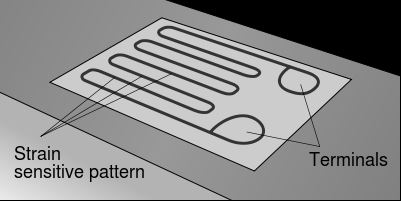
\includegraphics[width=0.5\textwidth]{billeder/Hardware/straingages1.JPG}
	\caption{illustration af strain gages}
	\label{fig:Strain gages}
\end{figure}
En strain gages modstand stiger ved stræk og falder ved kompression, dette kan beskrives ud fra formlen \ref{eq:modstandsformel}\citep{Websterbog}{s.47}
 \begin{align}
 R=\frac{P*L}{A}
 \label{eq:modstandsformel}
 \end{align}
 Hvor R=modstand, p=modstand per meter, L=længden og A=tværsnitsarealet. Der er mere til formlen en dette, bla. materiales egenskaber og temperatur. På vægtcellen er der fire strain gages, som er Placeret på vægtcellen på denne måde \ref{fig:Loadcell1}. Strain gages R1 og R4 bliver strukket, hvor R2 og R3 på undersiden bliver skubbet sammen.
 
 Måden de er forbundet er vist på \ref{fig:loadcell2}, denne metode at koble modstande på kaldes en wheatstone bro\citep{ELengbog}{s.122}. mere specifikt for denne er også kendt som et full-bridge kredsløb\citep{AETbog}{s.76}. Forholdet mellem input spændingen og output spændingen kan beskrives, som vist på \ref{eq:fullbformel}
\begin{align}
 V_{out}=GF*V_{in}*E
 \label{eq:fullbformel}
 \end{align}
 Hvor V$_{out}$=udgangssignalet, V$_{in}$=indgangsspændingen , GF=gages factor som er materialets egenskab og E=strukket der er tilført til vægtcellen.

\begin{figure}[htbp] \centering
\begin{minipage}[b]{0.48\textwidth} \centering
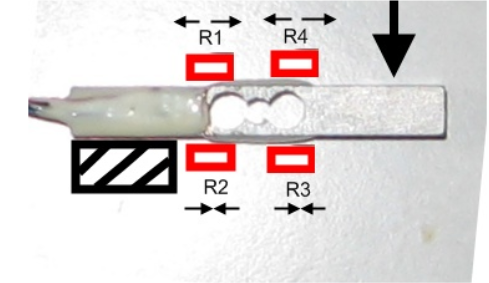
\includegraphics[width=1.00\textwidth]{billeder/Hardware/loadcell1.PNG} % Left picture
\end{minipage} \hfill
\begin{minipage}[b]{0.48\textwidth} \centering
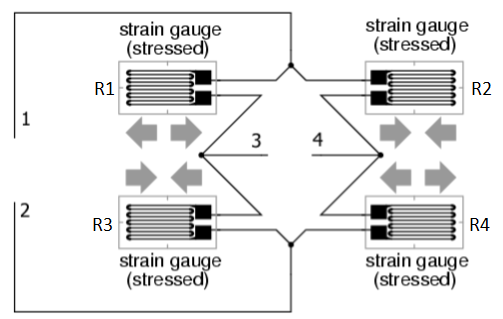
\includegraphics[width=1.00\textwidth]{billeder/Hardware/straingages2.PNG} % Right picture
\end{minipage} \\ % Captions og labels
\begin{minipage}[t]{0.48\textwidth}
\caption{illustration af strain gages i loadcell på virkning} % Left caption and label
\label{fig:Loadcell1}
\end{minipage} \hfill
\begin{minipage}[t]{0.48\textwidth}
\caption{illustration af koblingen strain gages i loadcell} % Right caption and label
\label{fig:loadcell2}
\end{minipage}
\end{figure}
Ud fra databladet \ref{subsec:loadcell} ses det, at output spændingen er 1.0mV pr volt på indgangsspændingen. Dette er pga. det meget lille strain der tilføres til emnet, hvilket også er med til at strain gagesene ikke går i stykker. Da Arduinoens analog til digital konverter bestående af 10bit, hvilket vil sige $2^{10}=1024$ det betyder at konverteren har 1024 trin fra 0 til 1023. Konverterens arbejdsspænding går fra 0 V til 5 V. 
\begin{align}
 \text{Spænding per trin}=\frac{\text{Maksimale spænding}}{\text{Antal trin}}=\frac{5 V}{1024\text{ trin}}=0,0049V=4,9mV
 \label{eq:volt-step}
 \end{align}
I \ref{eq:volt-step} viser det sig at den mindste værdi ADC kan måle er 4,9mV, dette medfører at arduinoen maksimal vil måle et step ved 1kg på vægtcellen, Da $1mV*5V=5mV$. Dette giver to valgmuligheder
\begin{enumerate}
\item Anskaffe en bedre ADC, bestående af flere bits
\item Hæve udgangsspændingen fra vægtcellen 
\end{enumerate}
I dette tilfælde vælges punkt 2, at hæve udgangsspændingen fra vægtcellen. 
\subsubsection*{Forstærkning af signal}
Til dette formål bruges en operationsforstærker, mere specifikt en differens operationsforstærker. En operationsforstærker består i sin mest simple funktion at forstærke et signal, men da udgangsspændingen fra vægtcellen er lav ønskes der følgende egenskaber:
\begin{enumerate}
\item En høj indgangsimpedans 
\item Differentielt input med et single ended output
\item En høj undertrykkelse af støj
\item En simple forstærkning
\end{enumerate}
Punkt 1, en høj indgangsimpedans (R$_{in}$ > 10-100M$\Omega$ ) sikre at forstærkeren ikke belaster måle objektet. Det ønskes for at få adgang til hele signalet, og at det ikke bliver undertrykt grundet at forstærkeren forbruger strømmen fra signalet.

Punkt 2, Differentielt input med et single ended output. Det er et ønske som skyldes at vægtcellen leverer et differentielt output. Hvor ved at et single ended output er lettere at arbejde med, især når der skal bruges en ADC. Indgangsmodstanden er bestemt ved modstanden mellem de to indgangsterminaler, som kan beskrives ved \ref{eq:differensmodstand} og beregnes ved \ref{fig:differensmodstand}
\begin{figure}[H]
	\centering
	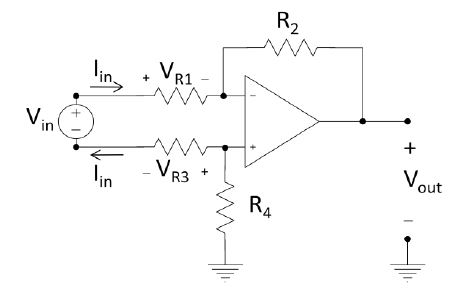
\includegraphics[width=0.5\textwidth]{billeder/Hardware/differensmodstand.JPG}
	\caption{illustration af differensforstærkerens indgangsmodstand}
	\label{fig:differensmodstand}
\end{figure}
\begin{align}
 R_{in} =V_{in}/I_{in}
 \label{eq:differensmodstand}
 \end{align}
I den ideelle verden antages det, at spændingsforskellen i mellem indgangsterminalerne er nul derfor kan der skrives vha. Kirchoffs spændingslov skrives i \ref{eq:differensmodstand2}
\begin{align}
 V_{R3}-V_{in}+V_{R1}=0=>V_{in}=V_{R3}+V_{R3}=I_{in}(R1+R3)=>R_{in}=\frac{V_{in}}{I_{in}=R1+R2}
 \label{eq:differensmodstand2}
 \end{align}
 I \ref{eq:differensmodstand2} viser det sig at indgangsmodstanden er beskrevet ved modstandene i det omkring liggende kredsløb. Hvilket giver anledning til at vælge så høje modstande som mulige, men store modstande øger risikoen for støj i kredsløbet. Det betyder at ønsket ikke kan opfyldes, med blot en differensforstærker


Punkt 3, en høj undertrykkelse af støj. Støj kan skyldes rigtig mange ting, en typiske støjkomponent er 50 Hz brum. 50 Hz brum fremkommer ofte, da støjen skyldes de omkring liggende EL installationer, hvor der foregår en elektromagnetisk kobling. men når der benyttes en differensforstærker, kan common mode støjen undertrykkes. Common mode støj er indstrålet støj der kommer på begge ledninger til differensforstærkeren. Det er differensforstærkeren god til at fra sorterer, fordi den trækker de to input fra hinanden. Det vil sige at hvis støjen er enes på de to ledninger, vil den differentiere den samme værdi fra hinanden hvilket vil give 0. en illustration af dette kan ses på \ref{fig:differensNoise} 
\begin{figure}[H]
	\centering
	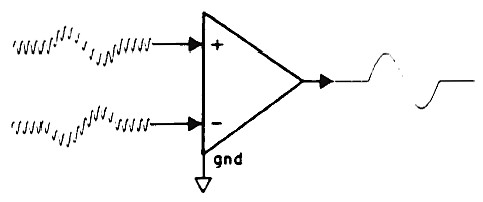
\includegraphics[width=0.5\textwidth]{billeder/Hardware/differensnoise.jpg}
	\caption{illustration af differensforstærkerens common mode støj undertrykkelse}
	\label{fig:differensNoise}
\end{figure}

Punkt 4, en simpel forstærkning. Med det over stående kredsløb, kan en simpel forstærkning ikke opnås. Det kan det ikke da det kræver at R2 divideret med R1 er lig med R4 divideret med R3. Hvilket vil være umuligt da modstande har en tolerancer for, hvor præcise de er.

For at opfylde de ønskede egenskaber skal differensforstærkeren modificeres. For at sikres en høj indgangsmodstand kan en spændingsføger benyttes, som har til formål at forstærke en til en. Det vil sige at den i teorien har samme udgangsspænding som indgangsspændingen. se \ref{fig:bufferamp} for en illustration, denne sættes på begge outputs fra vægtcellen.
\begin{figure}[H]
	\centering
	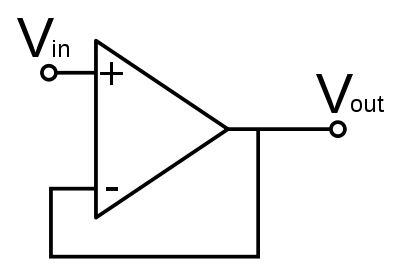
\includegraphics[width=0.5\textwidth]{billeder/Hardware/bufferamp.png}
	\caption{illustration af spændingsfølger}
	\label{fig:bufferamp}
\end{figure}
Med en spændingsfølger opnås der en høj indgangsmodstand, men signalet er stadig differentielt og uden forstærkning. Derfor indsættes der 3 modstande som vist i \ref{fig:bufferampmedgain}\citep{ASBbog}s.200
\begin{figure}[H]
	\centering
	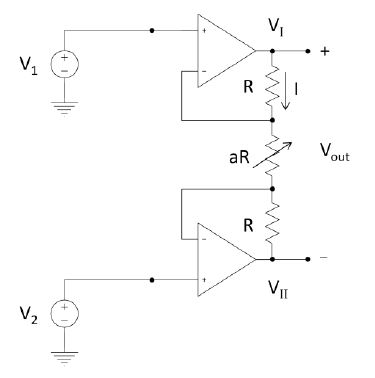
\includegraphics[width=0.5\textwidth]{billeder/Hardware/bufferampgain.JPG}
	\caption{illustration af spændingsfølger med gain}
	\label{fig:bufferampmedgain}
\end{figure}
Ved brug af KVL og KCL kan forstærkningen skrives som i \ref{eq:gain}, hvor $A_{d}$ er forstærkningen og $R_{a}$ er modstanden i midten. Dette gør forstærkningen simpel fordi der kun skal ændres en modstand. 
\begin{align}
 A_{d}=1+\frac{R+R}{R_{a}}
 \label{eq:gain}
 \end{align}
 Til at opfylde ønskerne om undertrykkelse af støj og et single ended output kan differensforstærkeren sættes efter spændingsfølgerne med forstærker trinet. Hvilket får kredsløbet til at se ud som vist i \ref{fig:bufferampmedgaindifferens}
 
 \begin{figure}[H]
	\centering
	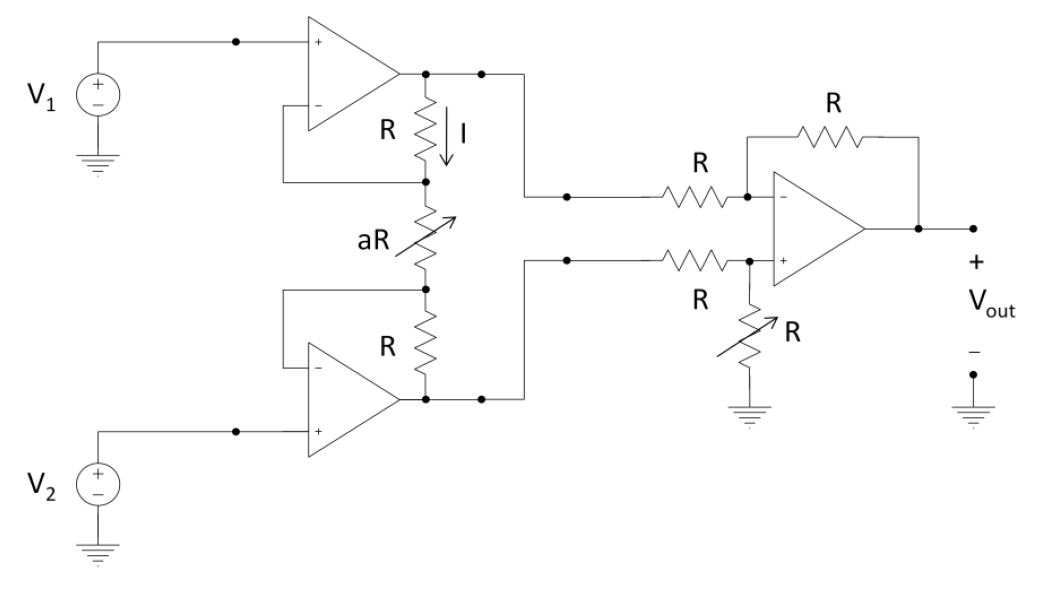
\includegraphics[width=0.5\textwidth]{billeder/Hardware/bufferampgaindifferens.JPG}
	\caption{illustration af spændingsfølger med gain og differensforstærker}
	\label{fig:bufferampmedgaindifferens}
\end{figure}

ligning \ref{eq:instru} viser overføringsfunktionen for diagrammet i \ref{fig:bufferampmedgaindifferens}.

\begin{align}
 V_{out}=(V_{2}-V_{1})*(1+\frac{R+R}{R_{a}})
 \label{eq:instru}
 \end{align} 
 
 Kredsløbet på \ref{fig:bufferampmedgaindifferens} kaldes en instrumentationsforstærker, hvilket der i projeket er indkøbt for at spare tid. Den indkøbte instrumentationsforstærker hedder INA114, som har kredsløbet- og pinkonfiguration vist på \ref{fig:INA114diagram} og \ref{fig:INA114Pin}\footnote{hentet fra databladet fra INA114}
 
 \begin{figure}[htbp] \centering
\begin{minipage}[b]{0.48\textwidth} \centering
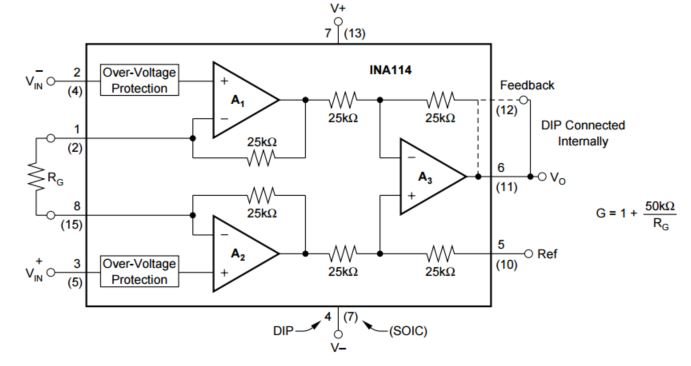
\includegraphics[width=1.00\textwidth]{billeder/Hardware/INA114diagram.JPG} % Left picture
\end{minipage} \hfill
\begin{minipage}[b]{0.48\textwidth} \centering
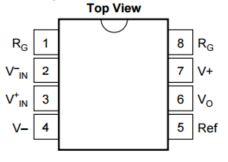
\includegraphics[width=1.00\textwidth]{billeder/Hardware/pinkonfig.JPG} % Right picture
\end{minipage} \\ % Captions og labels
\begin{minipage}[t]{0.48\textwidth}
\caption{INA114 diagram} % Left caption and label
\label{fig:INA114diagram}
\end{minipage} \hfill
\begin{minipage}[t]{0.48\textwidth}
\caption{pin konfiguration af INA114 8pin } % Right caption and label
\label{fig:INA114Pin}
\end{minipage}
\end{figure}
\fxnote{reference til datablad i billag}
Fra databladet til INA114 ses det at den har en CMRR på 115dB, ved et gain på 1000 og en indgangsmodstand på 10G$\Omega$. forstærkningen kan regnes ud fra formlen i databladet \ref{eq:gainina}
\begin{align}
 G=(1+\frac{50K\Omega}{R_{G}})
 \label{eq:gainina}
 \end{align} 
 I tilfældet i dette projekt skal der bruges et gain på $\frac{4,9V}{5mV}=980$, 4,9V for ikke at komme i mætning på arduinoens ADC og 5mV da det er den maksimale spænding vægtcellen kan give, ved 5V forsyning.
 \begin{align}
 R_{G}=\frac{50K\Omega}{980-1}=51\Omega
 \label{eq:gainina}
 \end{align}
Med et gain på 980 giver en $NY_{Maksimalespænding}=980*5mV=4,9V \pm0,147V$, dvs at der nu er en opløsning på
\begin{align}
 \frac{1000g}{trin}=\frac{1000g}{1024}=0,977g/trin=>0,977*\frac{1024}{5V}=200g/V \pm30g
 \label{eq:gainina}
 \end{align}
 kredsløbet for INA114 og vægtcellen til arduinoen kan ses på \ref{fig:loadcelldiagram}
 
  \begin{figure}[H]
	\centering
	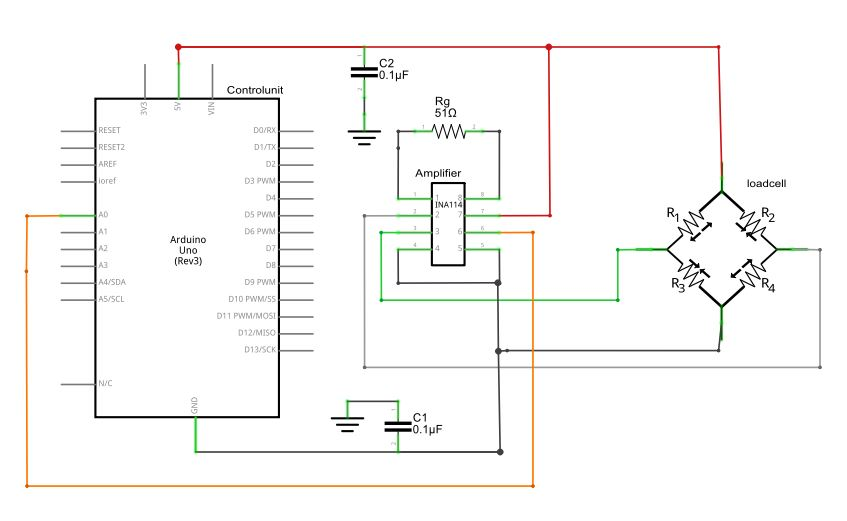
\includegraphics[width=0.9\textwidth]{billeder/Hardware/diagrammer/loadcelldiagram.JPG}
	\caption{Diagram for arduino, INA114 og vægtcelle}
	\label{fig:loadcelldiagram}
\end{figure}

Efter at diagrammet er fastlagt, testes forbindelserne nu på et \textit{fumlebræt} se \ref{fig:loadcelltest} for test opstilling
  \begin{figure}[H]
	\centering
	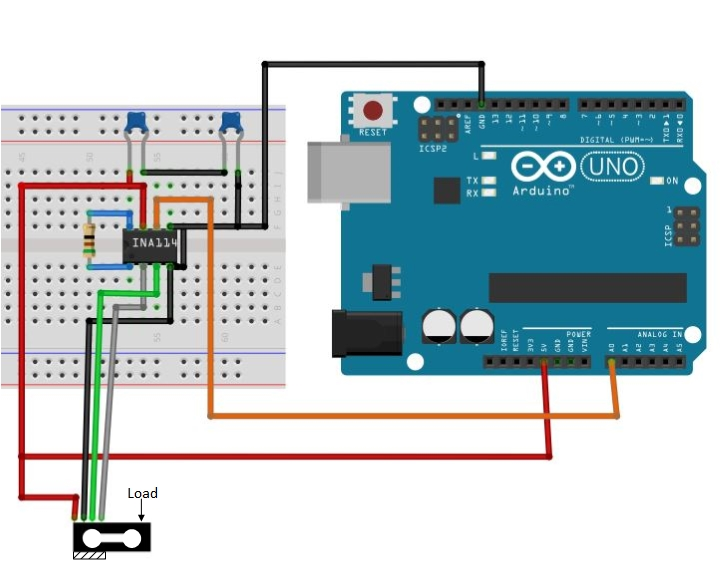
\includegraphics[width=0.9\textwidth]{billeder/Hardware/diagrammer/Drawing1.jpg}
	\caption{Test opstilling for vægtcelle}
	\label{fig:loadcelltest}
\end{figure}
 Se bilag\fxnote{reference til bilag} for at se testkode brugt i Arduino IDE til testopstilling for vægtcellen. Ved enhedstesten er der brugt et voltmeter til, at måle udgangsspændingen på ina114 for, at se om arduinoens ADC læste rigtigt. Til at sammenligne med voltmeteret, blev \ref{eq:trintilvolt} brugt til at konvertere ADC'ens bits værdi om til spænding.
 
 \begin{align}
 analogRead(A_0)*\frac{5}{1024}=\text{spænding i volt}
 \label{eq:trintilvolt}
 \end{align}
Den endelige opstilling af vægtcellen vil se ud som på \ref{fig:loadcell_mont} med celleopløsningsbeholder. I softwaren kræves det en kalibrering for at vægtcellen er præcis, dette er implementeret i \fxnote{reference til SW loadcell}
 
 \begin{figure}[H]
	\centering
	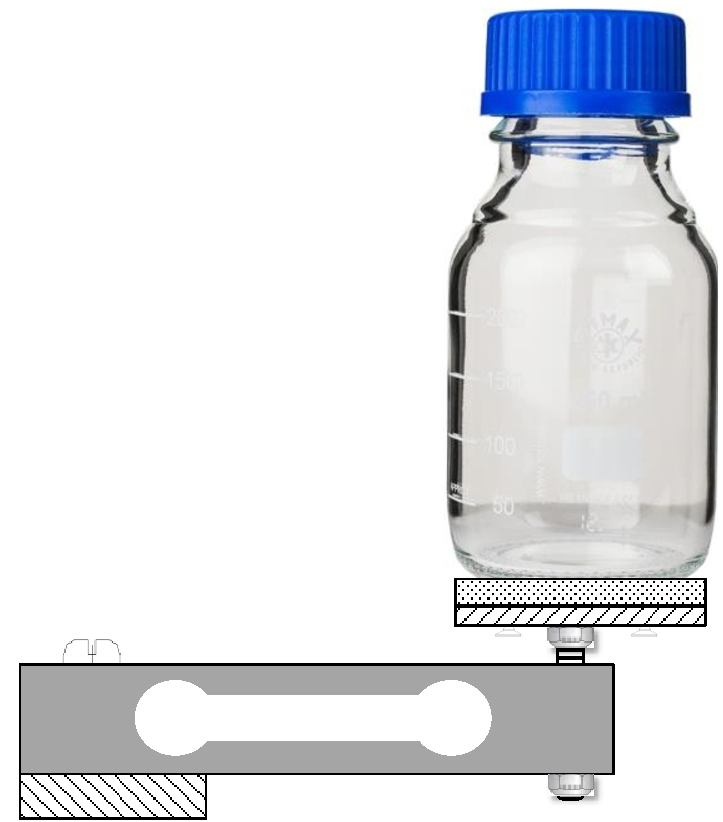
\includegraphics[width=0.5\textwidth]{billeder/Hardware/diagrammer/loadcell_montering.pdf}
	\caption{Illustration af opstilling med vægtcelle og celleopløsningsbeholder}
	\label{fig:loadcell_mont}
\end{figure}
 